%!TEX root =  FTL.tex
\appendix
\if0
\section{A minimax lower bound}
We prove a $\Omega(\log n)$ lower bound of the linear game in this section, when the adversary is constrained to have the average $\min_t \|\Theta_t\|_2 \ge L >0$.
The lower bound is achieved by computing the value of a particular linear game that satisfying the above constraint, thus serves as a lower bound for general linear games.

\begin{thm}
	Let $0<L\le 1/2$ and
	assume that $\min_t \|\Theta_t\|_2\ge L$ and let $\cW$ be the $\ell^2$ unit ball.
	Then for large enough $n$, $R_n = \Omega(\log (n)/L)$.
\end{thm}
The proof of \cref{thm:lowerbound} follows an idea due to \citet{abernethy2008optimal}: We compute the lower bound for each round backwards for $t=n,n-1,\dots,1$, by constructing a particular strategy for the adversary.

Let $\cW=\set{w}{\|w\|_2 \le r}$, $\cF = \set{f}{\|f\|_2\le 1}$, and $\cF_i = \set{f\in\cF}{\|\Theta_i\|_2\ge L}$ depending on $\{f_1, f_2, \ldots, f_{i-1}\}$. 
The value of the linear game is defined as follows:
\begin{align*}
V_n(\cW, \cF, L) & = \min_{w_1\in\cW}\max_{f_1\in\cF_1}\ldots\min_{w_1\in\cW}\max_{f_n\in\cF_n} \sum_{t=1}^{n} \inpro{f_t}{w_t} - \min_{w\in\cW} \sum_{t=1}^{n} \inpro{f_t}{w} \\
& = \min_{w_1\in\cW}\max_{f_1\in\cF_1}\ldots\min_{w_1\in\cW}\max_{f_n\in\cF_n} \sum_{t=1}^{n} \inpro{f_t}{w_t} +r \|F_{n-1} + f_n\|_2,
\end{align*}
where $F_t = \sum_{i=1}^{t}f_i$. 
Note that by further constraining the hypothesis set of the adversary, the value of the game $V_n(\cW, \cF, L)$ can be lowered bounded by 
\[
V_n \triangleq \min_{w_1\in\cW}\max_{f_1\in\tcF}\ldots\min_{w_1\in\cW}\max_{f_n\in\tcF} \sum_{t=1}^{n} \inpro{f_t}{w_t} +r \|F_{n-1} + f_n\|_2,
\]
where $\tcF = \set{f\in\cF}{\inpro{f}{\tau} \ge L}$ for some fixed unit vector $\tau$.

Our analysis follows the idea of \citep{abernethy2008optimal} to consider the optimal solution for each round reversely.
In particular, denote 
\[
g(F_{n-1}) = \min_{w\in\cW}\max_{f\in\tcF} \inpro{f}{w} +r \|F_{n-1} + f\|_2,
\] 
then $V_n$ satisfies
\[
V_n = \min_{w_1\in\cW}\max_{f_1\in\tcF}\ldots\min_{w_{n-1}\in\cW}\max_{f_{n-1}\in\tcF} \sum_{t=1}^{n-1} \inpro{f_t}{w_t} + g(F_{n-1}).
\]

The next result provides a lower bound of $g(F_{n-1})$.
\begin{prop}
	\label{prop:onestepoptimalgame}
	Let $F_t = \alpha_t\tau + \beta_t\tau^{\perp}_t$, where $\tau^{\perp}$ is a unit vector orthogonal to $\tau$ and $\beta_t >0$. Assume that $\alpha_t \ge tL$.
	Also assume that $\alpha_tL\ge\beta_t\sqrt{1-L^2}$ and $\alpha_t\sqrt{1-L^2}\ge\beta_tL$.
	Then 
	\[
	\min_{w\in\cW}\max_{f\in\tcF} \inpro{f}{w} + r\|F_t+f\|_2 \ge  \sqrt{\alpha_t^2 + 2\alpha_tL + 1+\beta_t^2} - \frac{\sqrt{\alpha_t^2+2\alpha_tL + 2\beta_t\sqrt{1-L^2} + 1}}{\sqrt{\alpha_t^2+2\alpha_tL + \beta_t^2 + 2\beta_t\sqrt{1-L^2} + 1}}L.
	\]
	Moreover, if $\alpha_t = tL$ and $\beta_t = \sqrt{t(1-L^2)}$, then
	\[
	\min_{w\in\cW}\max_{f\in\tcF} \inpro{f}{w} + r\|F_t+f\|_2 \ge r\|F_t\|_2 + \frac{1-L^2}{2Lt}+ \Omega(\frac{1}{t^2}).
	\]
	Finally, such lower bounds are achieved by picking $f = L\tau + \sqrt{1-L^2}u$ for some $u$ that is orthogonal to both $\tau$ and $\tau_t^\perp$.
\end{prop}



We now propose a strategy for the adversary such that a $\Omega(\log n)$ lower bound of $V_n$ is attained asymptotically.
The adversary plays $f_1 = L\tau + \sqrt{1-L^2}\tau_1^{\perp}$ for some arbitrary $\tau_1^{\perp}$ orthogonal to $\tau$. 
Then given $F_t$ decomposed as $ F_t= \alpha_t\tau + \beta_t \tau_t^{\perp}$ for some $\tau_t^{\perp}$ orthogonal to $\tau$, the adversary will play $f_{t+1}= L\tau + \sqrt{1-L^2}u$ for some $u$ that is orthogonal to both $\tau$ and $\tau_t^\perp$.
It is straightforward that by this strategy, $\alpha_t = tL$ and $\beta_t = \sqrt{t(1-L^2)}$.
Therefore, there exists a constant $N$, such that $\alpha_tL\ge \beta_t\sqrt{1-L^2}$, and $\alpha_t\sqrt{1-L^2}\ge \beta_tL$ for $t\ge N$ .

Therefore by \cref{prop:onestepoptimalgame}, the optimal solution for 
\begin{align*}
& \quad \min_{w_1\in\cW}\max_{f_1\in\tcF}\ldots\min_{w_n\in\cW}\max_{f_n\in\tcF} \sum_{t=1}^{n} \inpro{f_t}{w_t} +r \|F_{n-1} + f_n\|_2 \\
& \ge \min_{w_N\in\cW}\max_{f_N\in\tcF}\ldots\min_{w_n\in\cW}\max_{f_n\in\tcF} \sum_{t=N}^{n} \inpro{f_t}{w_t} +r \|F_{n-1} + f_n\|_2 + \Omega(1)\\
& = \min_{w_N\in\cW}\max_{f_N\in\tcF}\ldots\min_{w_{n-1}\in\cW}\max_{f_{n-1}\in\tcF} \sum_{t=N}^{n-1} \inpro{f_t}{w_t} + \min_{w_n\in\cW}\max_{f_n\in\tcF} \inpro{f_n}{w_n} +r \|F_{n-1} + f_n\|_2 \\
& \ge \min_{w_N\in\cW}\max_{f_N\in\tcF}\ldots\min_{w_{n-1}\in\cW}\max_{f_{n-1}\in\tcF} \sum_{t=N}^{n-1} \inpro{f_t}{w_t} + r\|F_{n-1}\|_2+\frac{1-L^2}{2Ln}+\Omega(\frac{1}{n^2})+\Omega(1) \\
& \ge \Omega(1)+ \frac{1-L^2}{2L}\sum_{t=N}^{n}\frac{1}{t} + \sum_{t=N}^{n}\Omega(\frac{1}{t^2}) + r\|F_{c-1}\|_2 \\
& =\Omega(\frac{\log n}{L}).
\end{align*}

\subsection{Proof of \cref{prop:onestepoptimalgame}}
Denote $w$ by $w = -p\tau + (-q)\tau_t^{\perp} + h u$, and $f$ by $f = a\tau + b\tau_t^{\perp}+cv$, where $u$ and $v$ are both unit vectors orthogonal to $\tau$ and $\tau_t^{\perp}$.
The optimization problem now becomes
\begin{align*}
& \quad \min_{p,q,h,u\,:\, p^2+q^2+h^2\le r^2}\, \max_{a,b,c,v\,:\, a\ge L, a^2+b^2+c^2\le 1} \inpro{f}{w} + r\|F_t+f\|_2 \\
& \equiv  \, \min_{p,q,h,u\,:\, p^2+q^2+h^2\le r^2}\, \max_{a,b,c,v\,:\, a\ge L, a^2+b^2+c^2\le 1} r\sqrt{(\alpha_t+a)^2 + (\beta_t+b)^2 + c^2} -pa -qb + hc\inpro{u}{v} \\
& \equiv  \, \min_{p,q,h\,:\, p^2+q^2+h^2\le r^2}\, \max_{a,b,c\,:\, a\ge L, a^2+b^2+c^2\le 1} r\sqrt{(\alpha_t+a)^2 + (\beta_t+b)^2 + c^2} -pa -qb + |h|c \numberthis\label{eq:eq31} \\
& \equiv  \, \min_{p,q\,:\, p^2+q^2\le r^2}\, \max_{a,b,c\,:\, a\ge L, a^2+b^2+c^2\le 1} r\sqrt{(\alpha_t+a)^2 + (\beta_t+b)^2 + c^2} -pa -qb \numberthis\label{eq:eq32}\\
& \equiv  r \, \min_{p,q\,:\, p^2+q^2\le 1}\, \max_{a,b,c\,:\, a\ge L, a^2+b^2+c^2\le 1} \sqrt{(\alpha_t+a)^2 + (\beta_t+b)^2 + c^2} -pa -qb \\
& \equiv  r \, \min_{p,q\,:\, p^2+q^2\le 1}\, \max_{a,b,c\,:\, a\ge L, a^2+b^2+c^2=1} \sqrt{(\alpha_t+a)^2 + (\beta_t+b)^2 + c^2} -pa -qb \numberthis\label{eq:eq33}\\
& \equiv  r \, \min_{p,q\,:\, p^2+q^2\le 1}\, \max_{a,b\,:\, a\ge L, a^2+b^2\le 1} \sqrt{\alpha_t^2+2\alpha_ta + \beta_t^2+2\beta_tb + 1} -pa -qb \\
& \equiv  r \, \min_{p,q\,:\,p\ge 0, q\ge 0, p^2+q^2\le 1}\, \max_{a,b\,:\, a\ge L, a^2+b^2\le 1} \sqrt{\alpha_t^2+2\alpha_ta + \beta_t^2+2\beta_tb + 1} -pa -qb \numberthis\label{eq:eq34}\\
& \triangleq r \, \min_{p,q\,:\,p\ge 0, q\ge 0, p^2+q^2\le 1}\, \max_{a,b\,:\, a\ge L, a^2+b^2\le 1} Q(p,q,a,b).
\end{align*}
Here Equation~\eqref{eq:eq31} is because the optimal $v$ is always picked to make $hc\inpro{u}{v} = |hc|$. Thus the optimal $h$ is $0$, leading to equation~\eqref{eq:eq32}. Then Equation~\eqref{eq:eq33} is due to the optimality of $c$.
We will first prove that the optimal solution $p^*$ and $q^*$ have to satisfy ${p^*}^2 + {q^*}^2 = 1. $
Let 
\[
p^*,q^*,a^*,b^* = \argmin_{p,q\,:\,p\ge 0, q\ge 0, p^2+q^2\le 1}\, \max_{a,b\,:\, a\ge L, a^2+b^2\le 1} Q(p,q,a,b),
\]
\[
\hat{a},\hat{b} = \argmax_{a,b\,:\, a\ge L, a^2+b^2\le 1} Q(\sqrt{1-{q^*}^2},q^*,a,b),
\]
and 
\[
\tilde{p},\tilde{q},\tilde{a},\tilde{b} = \argmin_{p,q\,:\,p\ge 0, q\ge 0, p^2+q^2= 1}\, \max_{a,b\,:\, a\ge L, a^2+b^2\le 1} Q(p,q,a,b).
\]
Thus, $Q(p^*,q^*,a^*,b^*) \le Q(\tilde{p},\tilde{q},\tilde{a},\tilde{b})$. On the other hand, $Q(p^*,q^*,a^*,b^*) \ge Q(p^*,q^*,\hat{a},\hat{b})$. Note that $\hat{a}\ge L > 0$, so $Q(p^*,q^*,\hat{a},\hat{b}) \ge Q(\sqrt{1-{q^*}^2}, q^*, \hat{a},\hat{b}) \ge Q(\tilde{p},\tilde{q},\tilde{a},\tilde{b})$.
Therefore, $Q(p^*,q^*,a^*,b^*) = Q(\sqrt{1-{q^*}^2}, q^*, \hat{a},\hat{b}) = Q(\tilde{p},\tilde{q},\tilde{a},\tilde{b})$, and the optimization problem is equivalent to 
\[
r \, \min_{p,q\,:\,p\ge 0, q\ge 0, p^2+q^2= 1}\, \max_{a,b\,:\, a\ge L, a^2+b^2\le 1} Q(p,q,a,b).
\]

Note that 
\begin{align*}
\frac{\partial Q}{\partial b}& =\frac{\beta_t}{\sqrt{\alpha_t^2+2\alpha_ta + \beta_t^2+2\beta_tb + 1}} - q; \\
\frac{\partial Q}{\partial a}& =\frac{\alpha_t}{\sqrt{\alpha_t^2+2\alpha_ta + \beta_t^2+2\beta_tb + 1}} - p.
\end{align*}
We compute the lower bound of Equation~\eqref{eq:eq34}, based on different cases of the value of $q$, as follows.\\

{\bf Case 1: $q\ge \frac{\beta_t}{\sqrt{\alpha_t^2+2\alpha_tL + \beta_t^2 - 2\beta_t\sqrt{1-L^2} + 1}}$.} \\
Note that in this case $\frac{\partial Q}{\partial b} \le 0$ for any $a,b$. Thus, the optimal $b^* = -\sqrt{1-{a^*}^2}$. Thus the optimization question is transformed to 
\[
\min_{p,q}\, \max_{a\,:\, 1\ge a\ge L} \sqrt{\alpha_t^2 + \beta_t^2+1+2\alpha_ta - 2\beta_t\sqrt{1-a^2}} -pa +q\sqrt{1-a^2}.
\]
It is straightforward that the optimal $q$ is the smallest possible $q$, i.e. $q^* = \frac{\beta_t}{\sqrt{\alpha_t^2+2\alpha_tL + \beta_t^2 - 2\beta_t\sqrt{1-L^2} + 1}}$.

{\bf Case 2: $q\le \frac{\beta_t}{\sqrt{\alpha_t^2 + \beta_t^2 +1 +2\sqrt{\alpha_t^2+\beta_t^2}}} = \frac{\beta_t}{\sqrt{\alpha_t^2+\beta_t^2}+1}$.} \\
Similar to Case 1, $\frac{\partial Q}{\partial b} \ge 0$, thus $b^* = \sqrt{1-a^*}$. The optimization problem is reduced to 
\[
\min_{p,q}\, \max_{a\,:\, 1\ge a\ge L} \sqrt{\alpha_t^2 + \beta_t^2+1+2\alpha_ta+2\beta_t\sqrt{1-a^2}} -pa  - q\sqrt{1-a^2}.
\]
Therefore, $q^* = \frac{\beta_t}{\sqrt{\alpha_t^2+\beta_t^2}+1}$.

{\bf Case 3: $\frac{\beta_t}{\sqrt{\alpha_t^2+\beta_t^2}+1} \le q \le \frac{\beta_t}{\sqrt{\alpha_t^2+2\alpha_tL + \beta_t^2 - 2\beta_t\sqrt{1-L^2} + 1}}$.} \\

Since $q \le \frac{\beta_t}{\sqrt{\alpha_t^2+2\alpha_tL + \beta_t^2 - 2\beta_t\sqrt{1-L^2} + 1}}$, 
\[p \ge \frac{\sqrt{\alpha_t^2+1+2\alpha_tL  - 2\beta_t\sqrt{1-L^2}}}{\sqrt{\alpha_t^2+2\alpha_tL + \beta_t^2 - 2\beta_t\sqrt{1-L^2} + 1}}
>\frac{\alpha_t}{\sqrt{\alpha_t^2+2\alpha_tL + \beta_t^2 - 2\beta_t\sqrt{1-L^2} + 1}}.
\]
Thus $\frac{\partial Q}{\partial a} \le 0$, and $a^* = L$. Therefore, the optimization problem is reduced into 
\[
\min_{p,q}\, \max_{b\,:\, b^2\le 1-L^2} \sqrt{\alpha_t^2+2\alpha_tL + \beta_t^2+2\beta_tb + 1} -pL -qb.
\]
{\bf SubCase 1: $\frac{\beta_t}{\sqrt{\alpha_t^2+\beta_t^2}+1} \le q \le \frac{\beta_t}{\sqrt{\alpha_t^2+2\alpha_tL + \beta_t^2 + 2\beta_t\sqrt{1-L^2} + 1}}$.} \\
Similarly, $\frac{\partial Q}{\partial b} = \frac{\beta_t}{\sqrt{\alpha_t^2+2\alpha_tL + \beta_t^2+2\beta_tb + 1}} - q \ge 0$, and thus $b^* = \sqrt{1-L^2}$. Solving 
\[
\min_{p,q}\, \max_{b\,:\, b^2\le 1-L^2} \sqrt{\alpha_t^2+2\alpha_tL + \beta_t^2+2\beta_t\sqrt{1-L^2} + 1} -pL -q\sqrt{1-L^2}.
\]
Further notice that by the constraints on $q$, 
\[
\frac{q}{p} \le \frac{\beta_t}{\sqrt{\alpha_t^2+2\alpha_tL + 2\beta_t\sqrt{1-L^2} + 1}}
\le \frac{\beta_t}{\alpha_t} \le \frac{\sqrt{1-L^2}}{L}.
\]
Therefore, $q^* = \frac{\beta_t}{\sqrt{\alpha_t^2+2\alpha_tL + \beta_t^2 + 2\beta_t\sqrt{1-L^2} + 1}}$. \\
{\bf SubCase 2: $\frac{\beta_t}{\sqrt{\alpha_t^2+2\alpha_tL + \beta_t^2 + 2\beta_t\sqrt{1-L^2} + 1}} \le q \le \frac{\beta_t}{\sqrt{\alpha_t^2+2\alpha_tL + \beta_t^2 - 2\beta_t\sqrt{1-L^2} + 1}}$.} \\
Note that given the constraint $p^2+q^2=1$, and the optimal solutions for $q^*$ in Case 1, Case 2, and SubCase 3, to solve the original problem Equation~\eqref{eq:eq34}, one only needs to consider SubCase 2.
Therefore, the original optimization problem becomes
\begin{align*}
& \quad \min_q \max_{b^2\le 1-L^2} \sqrt{\alpha_t^2+2\alpha_tL + \beta_t^2+2\beta_tb + 1} -\sqrt{1-q^2}L -qb \\ 
& \ge \min_q \sqrt{\alpha_t^2+2\alpha_tL + \beta_t^2 + 1} -\sqrt{1-q^2}L \\
& = \sqrt{\alpha_t^2 + 2\alpha_tL + 1+\beta_t^2} - \frac{\sqrt{\alpha_t^2+2\alpha_tL + 2\beta_t\sqrt{1-L^2} + 1}}{\sqrt{\alpha_t^2+2\alpha_tL + \beta_t^2 + 2\beta_t\sqrt{1-L^2} + 1}}L,
\end{align*}
where the first inequality is by picking $b=0$.

Plugging $\alpha_t = tL$ and $\beta_t = \sqrt{t(1-L^2)}$, by \cref{lem:onestepdiff}, 
\[
\min_{w\in\cW}\max_{f\in\tcF} \inpro{f}{w} + r\|F_t+f\|_2 \ge r\|F_t\|_2 + \frac{1-L^2}{2Lt}+ \Omega(\frac{1}{t^2}).
\]
\begin{lemma}
	\label{lem:onestepdiff}
	Given a fixed $L>0$, 
	\begin{align*}
	& \sqrt{n^2L^2+n(1-L^2)} - \sqrt{(n-1)^2L^2+(n-1)(1-L^2)}-\frac{\sqrt{n^2L^2+(1-L^2)+2\sqrt{n-1}(1-L^2)}}{\sqrt{n^2L^2+n(1-L^2)+2\sqrt{n-1}(1-L^2)}}L \\
	& = \frac{1-L^2}{2nL}+\Omega(\frac{1}{n^2}).
	\end{align*}
\end{lemma}
\begin{proof}
	Note that $\sqrt{x+\epsilon} = \sqrt{x}+\frac{\epsilon}{2\sqrt{x}}-\frac{\epsilon^2}{2x^{3/2}}+\Omega(\epsilon^3)$. Thus,
	\begin{align*}
	\sqrt{n^2L^2+n(1-L^2)} & = n\sqrt{L^2+\frac{1-L^2}{n}} \\ 
	& = n\left(L + \frac{\frac{1-L^2}{n}}{2L}-\frac{\left(\frac{1-L^2}{n}\right)^2}{4L^3} + O(\frac{1}{n^3})\right) \\
	& = nL + \frac{1-L^2}{2L} - \frac{(1-L^2)^2}{4nL^3} + O(\frac{1}{n^2}),
	\end{align*}
	and 
	\[
	\sqrt{(n-1)^2L^2+(n-1)(1-L^2)} = (n-1)L + \frac{1-L^2}{2L} - \frac{(1-L^2)^2}{4(n-1)L^3} + O(\frac{1}{n^2}).
	\]
	So 
	\[
	\sqrt{n^2L^2+n(1-L^2)} - \sqrt{(n-1)^2L^2+(n-1)(1-L^2)} = L + O(\frac{1}{n^2}).
	\]
	Therefore, it is sufficient to prove 
	\[
	L - \frac{\sqrt{n^2L^2+(1-L^2)+2\sqrt{n-1}(1-L^2)}}{\sqrt{n^2L^2+n(1-L^2)+2\sqrt{n-1}(1-L^2)}}L = O(\frac{1-L^2}{2nL}).
	\]
	\begin{align*}
	& \quad L - \frac{\sqrt{n^2L^2+(1-L^2)+2\sqrt{n-1}(1-L^2)}}{\sqrt{n^2L^2+n(1-L^2)+2\sqrt{n-1}(1-L^2)}}L \\
	& = \frac{\sqrt{n^2L^2+n(1-L^2)+2\sqrt{n-1}(1-L^2)} - \sqrt{n^2L^2+(1-L^2)+2\sqrt{n-1}(1-L^2)}}{\sqrt{n^2L^2+n(1-L^2)+2\sqrt{n-1}(1-L^2)}}L. \numberthis \label{eq:eq36}
	\end{align*}
	Similarly, 
	\begin{align*}
	\sqrt{n^2L^2+n(1-L^2)+2\sqrt{n-1}(1-L^2)} & = n\sqrt{L^2+\frac{n(1-L^2)+2\sqrt{n-1}(1-L^2)}{n^2}} \\
	&  = n\left(L + \frac{\frac{n(1-L^2)+2\sqrt{n-1}(1-L^2)}{n^2}}{2L} +O(\frac{1}{n^2})\right) \\
	& = nL + \frac{(1-L^2)+ \frac{2\sqrt{n-1}(1-L^2)}{n}}{2L} + O(\frac{1}{n}),
	\end{align*}
	and 
	\begin{align*}
	\sqrt{n^2L^2+(1-L^2)+2\sqrt{n-1}(1-L^2)} = nL+\frac{\frac{(1-L^2)+2\sqrt{n-1}(1-L^2)}{n}}{2L}+O(\frac{1}{n^2}).
	\end{align*}
	So Equation~\eqref{eq:eq36} equals
	\begin{align*}
	\frac{L}{\sqrt{n^2L^2+n(1-L^2)+2\sqrt{n-1}(1-L^2)}}\left( \frac{(n-1)(1-L^2)}{2nL}+O(\frac{1}{n})\right) = \frac{1-L^2}{2nL}+O(\frac{1}{n^2}).
	\end{align*}
\end{proof}
\fi
\section{More Lower Bounds}
\begin{thm}
	Let $\lambda \in (0,1/2)$ and $f(x) = 1 - \lambda x^2$ and $\mathcal F = \seto{(1,-1),(-1,-1)}$ and define a clipped ellipse with principal curvature $\lambda$ by 
	\begin{align*}
	\mathcal W = \seto{(x, y) : x \in [-1,1] \text{ and } 0 \leq y \leq f(x)}\,.
	\end{align*}
	Then for any strategy there exists a sequence of losses in $\mathcal F$ such that $R_n = \Omega\left(\frac{\log(n)}{\lambda}\right)$.
\end{thm}

\begin{proof}
	Let $U = \mathcal U([1/2-\lambda,1/2+\lambda])$ be a uniform distribution
	and suppose $P \sim U$ and let $X_1,\ldots,X_n$ be Bernoulli
	with mean $P$. Let $\ell_t = X_t (1,-1) + (1 - X_t)(-1,-1)$ so that $\ell^p = \Expc{\ell_t}{P=p} = (2p - 1, -1)$.
	Let $W_t \in \mathcal W$ be the choice of the strategy and so its loss in round $t$ is $\inner{W_t, \ell_t}$.
	Let $w^p = ((1 - 2p)/(2\lambda), f((1-2p)/(2\lambda)))$, which is the optimal choice when $P=p$. 
	
	Let $\hat P_{t-1} = \E[P|\ell_1 \ldots \ell_{t-1}]$ be the posterior mean after $t-1$ observations. 
	Then the Bayesian optimal choice in round $t$ is 
	\begin{align}
	\argmin_{w \in \mathcal W} \E\left[\inner{w, \ell^P}\Big| \ell_1\ldots\ell_{t-1}\right]
	&= \argmin_{w \in \mathcal W} \inner{w, \E[\ell^P|\ell_1 \ldots \ell_{t-1}]} \nonumber \\
	&= \argmin_{w \in \mathcal W} \inner{w, \ell^{\hat P_{t-1}}} \nonumber \\
	&= w^{\hat P_{t-1}}\,,
	\label{eq:bayes-opt}
	\end{align}
	where the first equality follows by linearity of the inner product, the second since $\ell^p$ is a linear function of $p$ and the third
	by the definition of $w^p$.
	Thus, we can bound the expected regret from below as
	\begin{align}
	\E[R_n] 
	&= \E\left[\max_{w \in \mathcal W} \sum_{t=1}^n \inner{W_t - w, \ell_t}\right]  
	\geq \max_{w \in \mathcal W} \E\left[ \sum_{t=1}^n \inner{W_t - w, \ell_t}\right] 
	= \E\left[\sum_{t=1}^n \inner{W_t - w^P, \ell_t} \right] \nonumber \\
	&= \E\left[\sum_{t=1}^n \inner{W_t - w^P, \ell^P} \right]
	= \sum_{t=1}^n \E\left[\E\left[\inner{W_t - w^P, \ell^P}\Bigg|\ell_1\ldots \ell_{t-1}\right]\right]\nonumber \\
	&\ge \sum_{t=1}^n \E\left[\min_w \E\left[\inner{w - w^P, \ell^P}\Bigg|\ell_1\ldots \ell_{t-1}\right]\right] \label{eq:bayes} \\
	&= \sum_{t=1}^n \E\left[\E\left[\inner{w^{\hat P_{t-1}} - w^P, \ell^P} \Bigg| \ell_1\ldots \ell_{t-1}\right]\right] 
	= \sum_{t=1}^n \E\left[\inner{w^{\hat P_{t-1}} - w^P, \ell^P} \right]\,, \nonumber
	\end{align}
	where  \cref{eq:bayes} follows since $W_t$ is chosen based on $\ell_1,\dots,\ell_{t-1}$ and the next equality follows 
	by \cref{eq:bayes-opt}.
	A simple calculation shows that $\big<w^q - w^p, \ell^p\big> = (p - q)^2 / \lambda$ for any $p, q \in [1/2-\lambda, 1/2+\lambda]$.
	Therefore the expected regret is lower bounded by
	\begin{align*}
	\E[R_n] 
	\geq \frac{1}{\lambda} \sum_{t=1}^n \E\left[\E\left[(\hat P_{t-1} - P)^2\Bigg|P\right]\right]
	= \Omega\left(\frac{\log(n)}{\lambda}\right)\,,
	\end{align*}
	where the second inequality follows from a version of the Bayesian central limit theorem. \todot{add reference, eg., Clarke and Barron, 1990, probably}
	The result is completed by noting that the worst-case regret is at least as big as the expected regret.
\end{proof}

\todot{check this}
\begin{remark}
	As $n$ tends to infinity the exact constant (for this prior) is
	\begin{align*}
	\lim_{n\to\infty} \frac{R_n}{\log(n)} \geq \frac{1}{\lambda} \int^{1/2+\lambda}_{1/2-\lambda} p(1-p) dU(p) = \frac{1}{4\lambda} - \frac{\lambda}{3}\,.
	\end{align*}
\end{remark}

\section{Adaptive Algorithms for the Unit Ball Constraint Set}

In this section we provide some interesting results about adaptive algorithms for the case when $\cW$ is the unit ball in $\R^d$ (naturally, the results easily generalize to any ball centered at the origin). First, we show that a variant of FTL using shrinkage as regularization has $O(\log(n))$ regret when $\|\Theta_t\|_2 \ge L>0$ for all $t$, but it also has $O(\sqrt{n})$ worst case guarantee. Furthermore, we show that the standard FTRL algorithm is adaptive if the constraint set is the unit ball and the loss vectors are stochastic.
Throughout the section we will use the notation $F_t=-(t-1)\Theta_t=\sum_{i=1}^{t-1} f_t$.

\subsection{Follow the Shrunken Leader}

In this section we are going to analyze a combination of the FTL algorithm and the idea of shrinkage often used for regularization purposes in statistics. We assume that $\cW=\set{x \in \R^d}{ \|x\|_2 \le 1}$ is the unit ball and,  without loss of generality, we further assume that $\|f\|_2 \le 1$ for all $f\in\cF$. 
	\begin{algorithm}[t]
		\caption{Follow The Shrunken Leader (FTSL}
		\label{alg:adaptiveAlgorithm}
		\begin{algorithmic}[1]
			\STATE Predict $w_1 = 0$; 
			\FOR {$t = 2, ..., n-1$}
			\STATE {FTL: Compute $\tilde{w}_{t} = \argmin_{w\in\cW} \inner{ w, F_{t-1}}$}
			\STATE {Shrinkage: Predict $w_t = \frac{\|F_{t-1}\|_2}{\sqrt{\|F_{t-1}\|_2^2+t+2}}\tilde{w}_{t}$}
			\ENDFOR
			\STATE {FTL: Compute $\tilde{w}_{n} = \argmin_{w\in\cW} \inner{ w, F_{n-1}}$}
			\STATE {Shrinkage: Predict $w_n = \frac{\|F_{n-1}\|_2}{\sqrt{\|F_{n-1}\|_2^2+n}}\tilde{w}_{n}$}
		\end{algorithmic}
	\end{algorithm}
\begin{thm}
 
 The Follow The Shrunken Leader (FTSL) algorithm is given in \cref{alg:adaptiveAlgorithm}. The main idea of the algorithm is to predict a shrunken version of the FTL prediction, in this way keeping it away from the boundary of $\cW$. The next theorem shows that the right amount of shrinkage leads to a robust, adaptive algorithm:
  \begin{itemize}
 	\item If there exists $L$ such that $\|\Theta_t\|_t \ge L>0$ for $1\le t\le n$, then the regret of FTSL is $O(\log(n)/L)$.
 	\item Otherwise, the regret of FTSL is at most $O(\sqrt{n})$.
 \end{itemize}
\end{thm}
\begin{proof}
	By the definition of $F_t$ and $\cW$, $\tilde{w}_{t} =- F_{t-1}/\|F_{t-1}\|_2$.
	Let $\sigma_n = \frac{\|F_{n-1}\|_2}{\sqrt{\|F_{n-1}\|_2^2 + n}}$.
	Our proof follows the idea of \citet{abernethy2008optimal}. We compute the upper bound on the value of the game for each round backwards for $t=n,n-1,\dots,1$, by solving the optimal strategies for $f_t$.
	The value of the game using FTSL is defined as
	\begin{align*}
	V_n & = \max_{f_1, \ldots, f_n} \sum_{t=1}^{n}\inpro{w_t}{f_t}- \min_{w\in\cW} \inpro{w}{F_n} \\
	& = \max_{f_1,\ldots, f_{n-1}} \sum_{t=1}^{n-1}\inpro{w_t}{f_t} + \underbrace{\max_{f_n} \|F_{n-1}+f_n\|_2 + \inpro{f_n}{w_n}}_{=:U_n}
	\end{align*}
We first prove that $U_n$, the second term above, is bounded from above by  $\sqrt{\|F_{n-1}\|_2^2 + n}$. To see this, let $f_n = a_n \tilde{F}_{n-1} + b_n \Omega_{n-1}$ where $\tilde{F}_{n-1}$ is the unit vector parallel to $F_{n-1}$ and $\Omega_{n-1}$ is a unit vector orthogonal to $F_{n-1}$.  Furthermore, since $\|f_n\|_2 \le 1$, we have $a_n^2+b_n^2 \le 1$.
Thus,
\begin{align*}
U_n & = \max_{f_n} \sqrt{\|F_{n-1}\|_2^2 + 2a_n\|F_{n-1}\|_2 + a_n^2 + b_n^2} - a_n\sigma_{n}\\
 & \le \max_{a} \sqrt{\|F_{n-1}\|_2^2 + 2a\|F_{n-1}\|_2 + n} - a\sigma_{n}\\
 & = \sqrt{\|F_{n-1}\|_2^2 + n},
\end{align*}  
where the last equality follows since the maximum is attained at $a=0$. 
A similar statement holds for the other time indices: for any $t \ge 1$,
\begin{equation}
\label{eq:stepDiff1}
\max_{f_t} \sqrt{\|F_{t-1} + f_t\|_2^2 + t + 1} + \inpro{f_t}{w_t} \le  \sqrt{\|F_{t-1}\|_2^2 + t} + \frac{1}{\sqrt{t}}~.
\end{equation}
Before proving this inequality, let us see how it implies the second statement of the theorem:
\begin{align*}
V_n & \le \max_{f_1,\ldots, f_{n-1}} \sum_{t=1}^{n-1}\inpro{w_t}{f_t} + \sqrt{\|F_{n-1}\|_2^2 + n} \\
& \le \max_{f_1,\ldots, f_{n-2}} \sum_{t=1}^{n-2}\inpro{w_t}{f_t}  + \sqrt{\|F_{n-2}\|_2^2 + n-1} + \frac{1}{\sqrt{n}} \\
& \le \ldots \\
& \le 1+ \sum_{t=1}^{n}\frac{1}{\sqrt{t}} = O(\sqrt{n}).
\end{align*}
Moreover, if $\|\Theta_t\|_2 \ge L$ for $1\le t\le n$, a stronger version of \eqref{eq:stepDiff1} also holds:
\begin{equation}
\label{eq:stepDiff2}
\max_{f_t} \sqrt{\|F_{t-1} + f_t\|_2^2 + t + 1} + \inpro{f_t}{w_t} \le  \sqrt{\|F_{t-1}\|_2^2 + t} + \frac{1}{(t-1)L}.
\end{equation}
This implies the first statement of the theorem, since
\begin{align*}
V_n & \le \max_{f_1,\ldots, f_{n-1}} \sum_{t=1}^{n-1}\inpro{w_t}{f_t} + \sqrt{\|F_{n-1}\|_2^2 + n} \\
& \le \max_{f_1,\ldots, f_{n-2}} \sum_{t=1}^{n-2}\inpro{w_t}{f_t}  + \sqrt{\|F_{n-2}\|_2^2 + n-1} + \frac{1}{(n-1)L} \\
& \le \ldots \\
& \le 1+ \sum_{t=1}^{n-1}\frac{1}{tL} = O(\log(n)/L).
\end{align*}

To finish the proof, it remains to show \eqref{eq:stepDiff1} and \eqref{eq:stepDiff2}.
Let  $f_t = a_t \tilde{F}_{t-1} + b_t \Omega_{t-1}$ where $\tilde{F}_{t-1}$ is the unit vector parallel to $F_{t-1}$ and $\Omega_{t-1}$ is a unit vector orthogonal to $F_{t-1}$. Since $\|f_t\|_2 \le 1$, observe that $a_t^2+b_t^2 =\|f_t\|_2 \le 1$. Furthermore, let $\sigma_t = \frac{\|F_{t-1}\|_2}{\sqrt{\|F_{t-1}\|_2^2 + t+2}}$.
Then, for any $t \ge 1$,
	\begin{align}
	\Delta_t & =\max_{f_t} \sqrt{\|F_{t-1}\|_2^2 + 2a_t\|F_{t-1}\|_2 + a_t^2 + b_t^2 + t+1} - a_t\sigma_t  - \sqrt{\|F_{t-1}\|_2^2 + t}  \nonumber\\
	& \le \max_{a_t} \sqrt{\|F_{t-1}\|_2^2 + 2a_t\|F_{t-1}\|_2 + t+2} - a_t\sigma_t  - \sqrt{\|F_{t-1}\|_2^2 + t}  \nonumber\\
	& = \sqrt{\|F_{t-1}\|_2^2 + t+2} - \sqrt{\|F_{t-1}\|_2^2 + t}  \nonumber\\
	& = \frac{2}{\sqrt{\|F_{t-1}\|_2^2 + t+2} + \sqrt{\|F_{t-1}\|_2^2 + t}} \label{eq:stepDiff3} \\
	& \le \frac{1}{\sqrt{t}}. \nonumber
	\end{align}
	This proves \eqref{eq:stepDiff1}.
	Moreover, if $\|F_{t-1}\|_2 = \|(t-1)\Theta\|_2 \ge (t-1)L$, by \eqref{eq:stepDiff3} we obtain
	\[
	\Delta_t \le \frac{2}{\sqrt{\|F_{t-1}\|_2^2 + t+2} + \sqrt{\|F_{t-1}\|_2^2 + t}} \le \frac{1}{\|F_{t-1}\|_2}\le \frac{1}{(t-1)L},
	\]
	proving \eqref{eq:stepDiff2}.
\end{proof}


\subsection{FTRL for the case of the unit ball constraint set}
This section is to show that in the case when $\cW$ is the unit ball in $\ell_2$ norm, FTRL  with $R(w) = \frac{1}{2}\|w\|^2$ as its regularization is an adaptive algorithm. To fix the notation, in round $t$, FTLR predicts
\[
	w_{t} = \argmin_{w\in \cW} \eta_t \inpro{F_{t-1}}{w} + R(w), 
\]
if $t >1$ and $w_1=0$.
It has been well known that FTRL with $\eta_t = 1/\sqrt{t-1}$ is guaranteed to achieve $O(\sqrt{n})$ regret in the adversarial setting, see, e.g., \citep{SS12:Book}. It remains to prove that FTRL indeed achieves a fast rate in the stochastic setting. 
\begin{thm}
	Assume that the sequence of loss vectors, $f_1,\ldots,f_n \in \R^d$  satisfies $\|f_t\|_2 \le 1$ almost surely and $\Exp{f_t} = \mu$ for all $t$ with some $\|\mu\|_2 >0$. Then FTRL with $\eta_t=1/\sqrt{t-1}$ suffers $O(\log n)$ regret .
\end{thm}

\begin{proof}
	Using $R(w) = \frac{1}{2}\|w\|^2$ as its regularization, in round $t>1$ FTRL predicts 
	\begin{equation}
	\label{eq:ftrl-eq}
	w_{t} = \argmin_{w\in \cW} \eta_t \inpro{F_{t-1}}{w} + R(w) = 
	\begin{cases}
	\frac{1}{\sqrt{t-1}} F_{t-1} & \quad \text{if  } \|F_{t-1}\| \le \sqrt{t-1} \\
	\frac{F_{t-1}}{\|F_{t-1}\|} & \quad \text{otherwise.} 
	\end{cases}
	\end{equation}
	For any $1\le t \le n$,  denote the event $\|F_t\| \ge \sqrt{t}$ by $\cE_t$. Note that if $\|F_{t-1}\| \ge \sqrt{t-1}$, FTRL predicts exactly the same $w_t$ as FTL. Denote the accumulate loss of FTL in $n$ rounds by $\cL^{FTL}_n$. Thus, the regret of FTRL is
	\begin{align*}
	\Exp{R_n} & = \Exp{\sum_{t=1}^{n} \inpro{f_t}{w_t} - \min_{w\in\cW}  \inpro{f_t}{w}} \\
	& = \Exp{ \sum_{t=1}^{n} \inpro{f_t}{w_t} - \cL^{FTL}_n }+ \Exp{\cL^{FTL}_n - \min_{w\in\cW} \inpro{f_t}{w} } \\
	& \le 2 \sum_{t=1}^{n} \Prob{\cE_t^c} + O(\log n),
	\end{align*}
	where, to obtain the last inequality, we applied \eqref{eq:ftrl-eq} for the first term, while the second term is $O(\log n)$ by the discussion following \cref{thm:R_curvesurface}.
	It remains to bound the first term, 2 $\sum_{t=1}^{n} \Prob{\cE_t^c} $ in the above.
	For any $t > \frac{4}{\|\mu\|_2^2}$,
	\begin{align*}
	\Prob{ \|F_{t}\|_2 \le \sqrt{t} } &\le \Prob{ \|F_{t}\|_2 <  \frac{t}{2}\|\mu\|_2 } \le \sum_{i=1}^d \Prob{|F_{t,i}| < \frac{t}{2} |\mu_i|} \\
	             &\le \sum_{i=1}^d \Prob{|F_{t,i}-t\mu_i| >  \frac{t}{2} |\mu_i|} \le 2 \sum_{i=1}^d e^{-\frac{\mu_i^2}{4} t}
	\end{align*}
	Thus,
	\begin{align*}
	\sum_{t=1}^{n} \Prob{\cE_t^c}  & = \sum_{t=1}^{4/\|\mu\|_2^2} \Prob{\cE_t^c}  + \sum_{t=4/\|\mu\|_2^2}^{n} \Prob{\cE_t^c} \\
	& \le \frac{4}{\|\mu\|_2^2} + 2\sum_{i=1}^d \sum_{t=0}^{n} e^{-\frac{\mu_i^2}{4} t} \\
	& \le \frac{4}{\|\mu\|_2^2} + 2\sum_{i=1}^d \frac{1}{1-e^{ -\frac{\mu_i^2}{4}}} \\
	& \le  \frac{4}{\|\mu\|_2^2} + 2\sum_{i=1}^d \frac{\mu_i^2}{4} = \frac{4}{\|\mu\|_2^2}  + \frac{\|\mu\|_2^2}{2}~.
	\end{align*}
	where in the last inequality we used $1/(1-e^{-a}) \le a$.
	Therefore, if $\|\mu\| > 0$, the regret of FTRL satisfies
	\[
	\Exp{R_n} \le \frac{8}{\|\mu\|_2^2} + \|\mu\|_2^2 + O(\log n) = O(\log n).
	\]
\end{proof}

We close this section by comparing the performance of our different adaptive algorithms on a synthetic example. We compare FTL, FTSL, FTLR, and AB(FTL,FTRL). All these algorithms are parametrized as above. The problem setup is similar to the stochastic data setting in \cref{sec:Simulations}. Again, we consider a 4-dimensional setting, that is, $\cW$ is the unit ball in $\R^4$ centered at the origin.
We sample the i.i.d. vectors $\hat{f}_t$ from a zero-mean normal distribution with independent components whose variance is $1/16$, and let $\tilde{f_t}=\hat{f}_t$ if $\|\hat{f}_t\|_2 \le 1$ and $\tilde{f}_t = \hat{f}_t/\norm{\hat{f}_t}_2$ when $\norm{\hat{f}_t}_2>1$.
The reason of this modification is to encourage the occurrence of the event $\|F_{t-1}\|_2 < \sqrt{t-1}$. Recall that when $\|F_{t-1}\|_2 \ge \sqrt{t-1}$, the prediction of FTRL matches that of FTL, so we are trying to create some data where their behavior is actually different. As a result, we will be able to observe that the predictions of FTL and FTRL are different in the early rounds. Finally, as before, we let $f_t=\tilde{f}_t + L e_1$, and set the time horizon to $n=20,000$.
 

The results of the simulation are shown in Figure~\ref{res:Stoc_unitBall}. In the case of $L=0.1$, FTRL suffers more regret at the beginning for some rounds, but then succeeds to match the performance of FTL.

\begin{figure}[h]
	\centering
	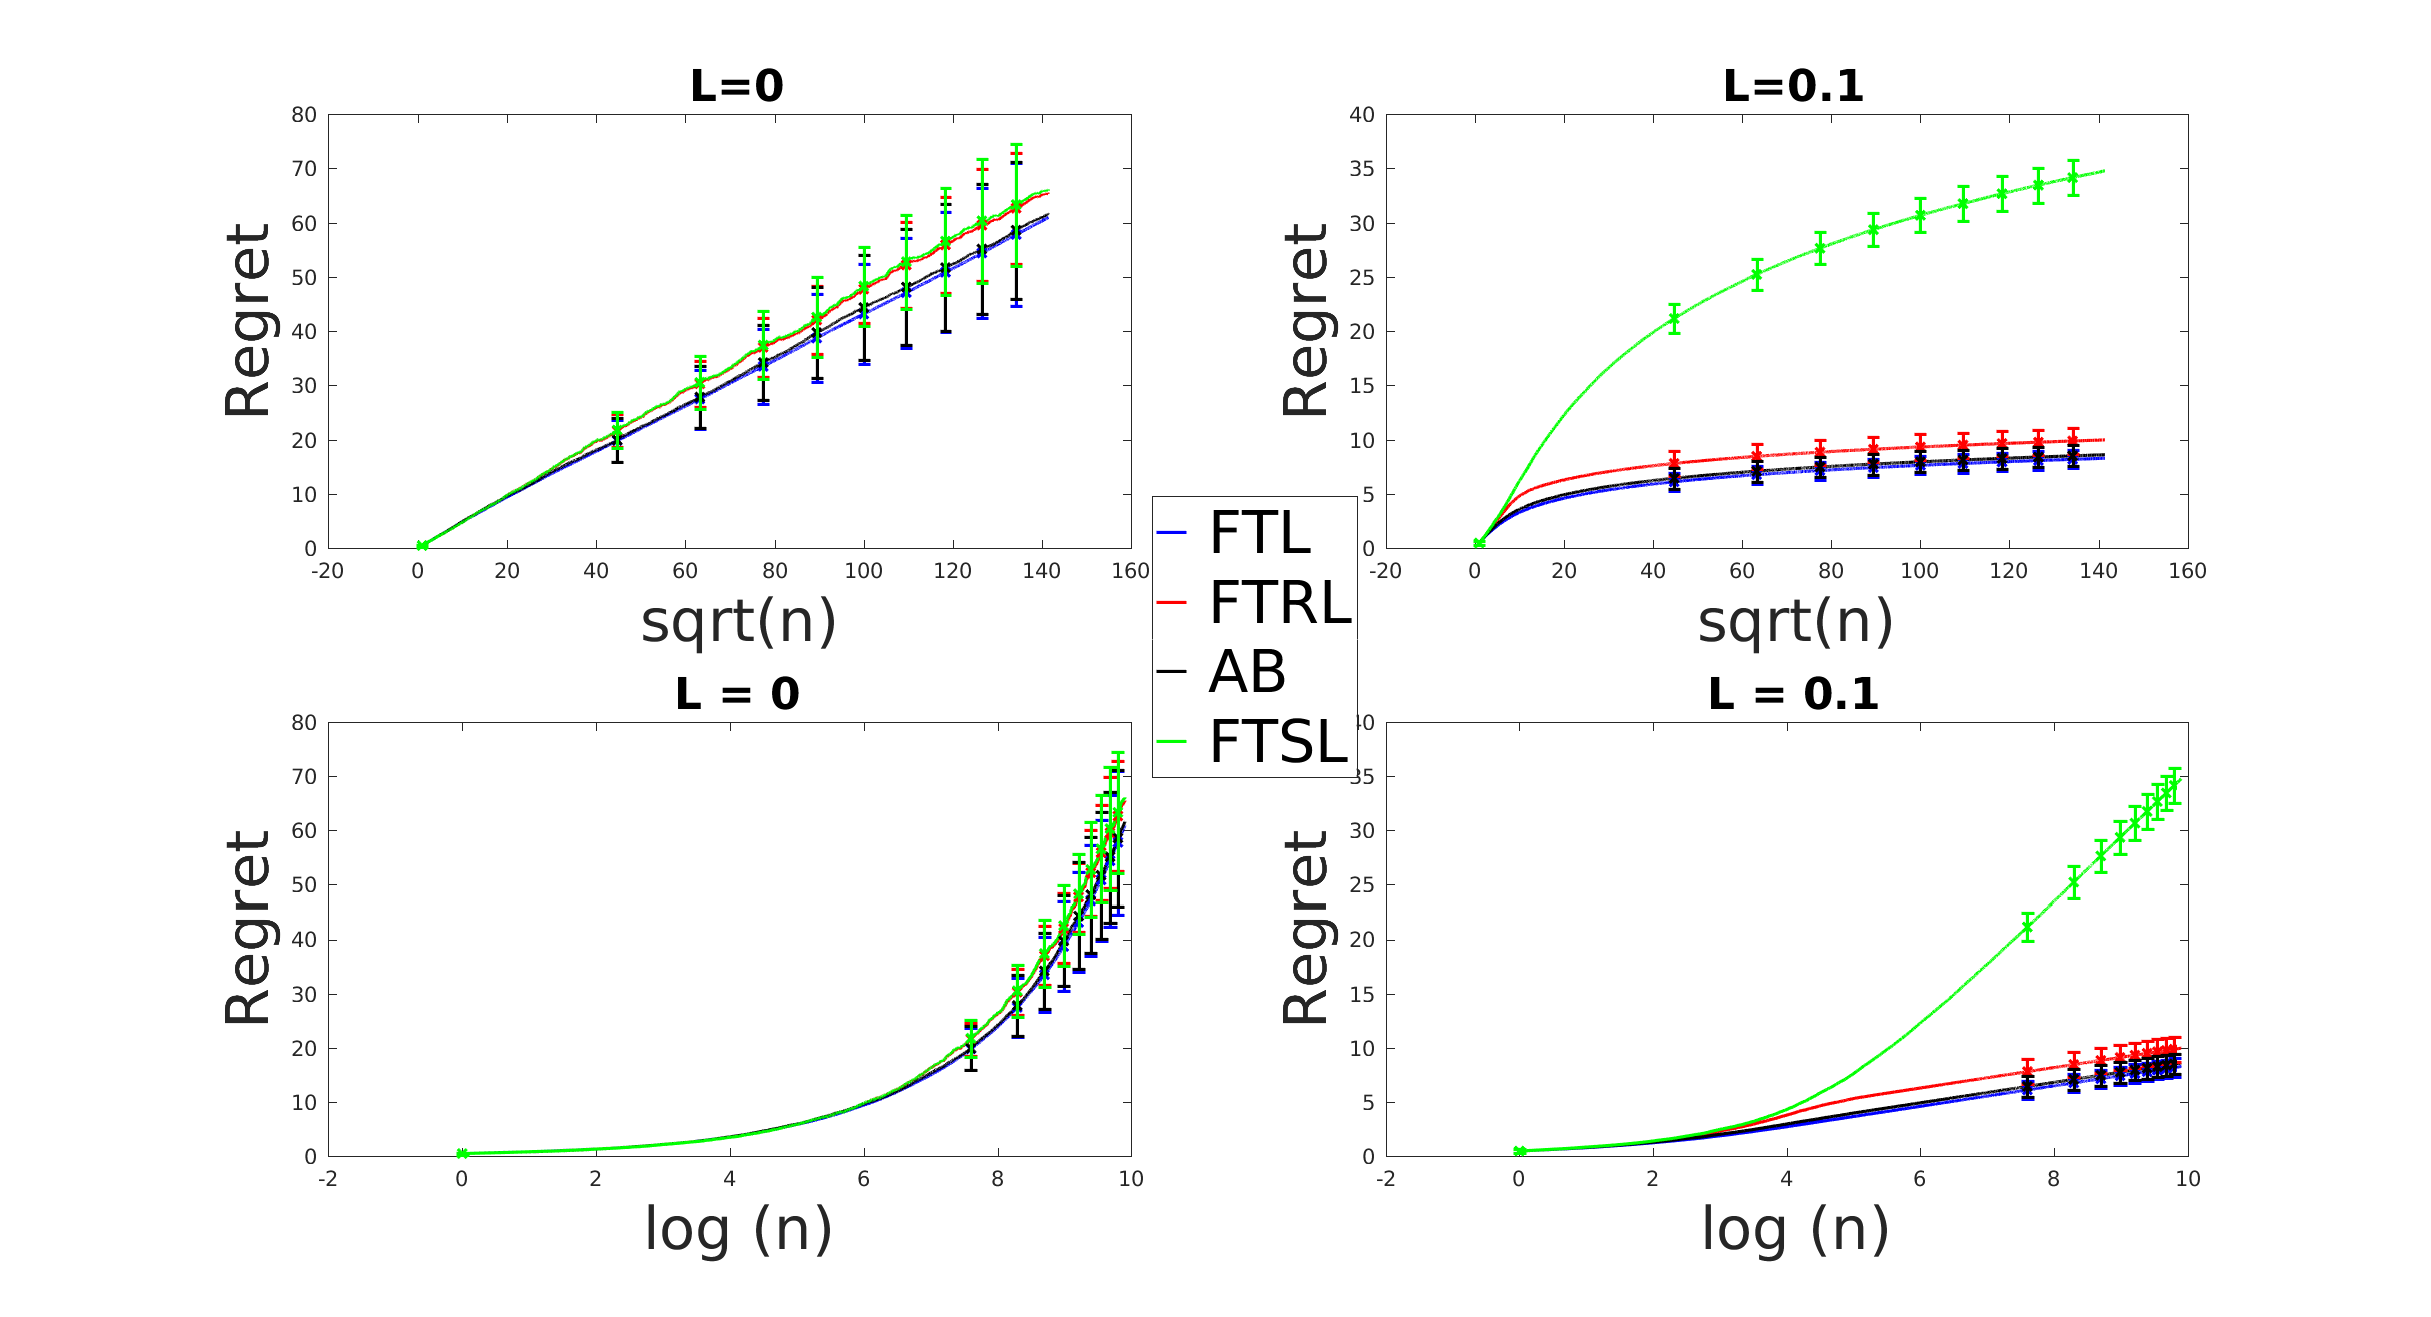
\includegraphics[height = 5cm]{figures/ExpResults/Stoc_unitBall}	
	\caption{Experimental results for stochastic data. \label{res:Stoc_unitBall}}
\end{figure}


\if0
\section{An adaptive Algorithm for the Linear Game}
\todor[inline]{The idea of shrinking the original estimation does not work so far. It requires $\frac{\|f_t\|}{\|\Theta_{t-1}\|}$ or $\frac{\|\Theta_t\|}{\|\Theta_{t-1}\|}$ to be small to have a $O(\sqrt{n})$ regret in the worst-case data.}
In order to achieve the $O(\log(n))$ regret in \cref{thm:R_curvesurface}, condition $\| \Theta_t\|_2 \ge L >0$ is necessary. 
In fact, A $O(\sqrt{n})$ lower bound of the linear game has been proved of \citet{abernethy2008optimal} when $\cW$ is a ball in the Euclidean space.
The "follow the regularized leader" algorithm (FTRL) attains a $O(\sqrt{n})$ regret, thus achieves the optimal rate for the worst-case data.
However, it is easy to see that FTL may suffer a trivial $O(n)$ regret for the worst-case data, whereas FTRL has $O(\sqrt{n})$ regret even for the easy data where FTL will performs much better.

This phenomenon raise a natural question: can we have an algorithm that can adapt to difficulty of the data, and thus achieve $O(\log(n))$ regret when the data is easy, while only suffer $O(\sqrt{n})$ regret when the data is difficult.
Results about such adaptive algorithm is not new in the literature \citep{sani2014exploiting,bubeck2012best}. 
In this section we present a new adaptive algorithm for the linear game. Compared to the (A,B)-prod algorithm in \citep{sani2014exploiting}, our algorithm is simpler without running both FTL and FTRL in each round. 
%Our algorithm also provides a continuous transition between the easy data and the worst data, while the resulting regret in the (A,B)-prod algorithm is in a binary style, either being $O(\sqrt{n\log(n)})$ or $\O(\log(n))$.\todoa{This sentence is absolutely not justified, and I don't think it is true in general! It should be removed.}
Finally, the regret of our algorithm for the worst-case data is $O(\sqrt{n})$, matching the lower bound, while the regret of (A,B)-prod is $O(\sqrt{n\log(n)})$.

The worst case sequence presented in the lower bound of \citet{abernethy2008optimal} keeps the sequence $(\Theta_t)$ close to the origin, and the FTRL algorithm achieves the optimal regret rate by penalizing larger values of $w_t$, keeping it away from the boundary of $\cW$. To mimic this idea, we shrink the prediction $w_t$ of FTL towards zero based on the magnitude of $\|\Theta_{t-1}\|$: for larger values of $\Theta_{t-1}$ we do not need to shrink at all, but for small values we need to keep the prediction small to avoid potentially large losses for a changing sequence $f,-f,f,-f,\ldots$ of losses. 

We assume that $\cW$ is of a star shape, that is, $c w\in\cW$ for any $0 \le c \le1$ and $w\in\cW$. 
% and for simplicity we assume that $\|w\|_2 \le 1$ for all $w \in \cW$. 
Define the shrinkage function
for any $t \ge 1$ and $\theta \ge 0$ as the centered sigmoid function
\[
\sigma_t(\theta)= \frac{1-e^{-\theta\sqrt{t+1}}}{1+e^{-\theta\sqrt{t+1}}}~.
\]

Given $\sigma_t$, our regularized prediction algorithm, called Follow The Shrunken Leader (FTSL), is defined as follows:
\begin{algorithm}[H]
	\caption{Shrinked FTL}
	\label{alg:FTSL}
	\begin{algorithmic}[1]
		\STATE $w_1 = 0$
		\FOR{$t = 2 \text{ to } n$} 
		\STATE Compute the prediction by FTL $w_t =  \argmin_{w\in\cW} \sum_{i=1}^{t-1} \ip{ w, f_i }$.
		\STATE The learner predicts $\tw_t = \sigma_{t-1}(\|\Theta_{t-1}\|) w_t \in \cW$.  % (Note that $\tw_t \in \cW$.)
		\ENDFOR
	\end{algorithmic}
\end{algorithm}

\begin{prop}
	Let $M = \max_{f\in \cF} \norm{f}_2$.
	Assume that the principal curvatures of the surface $\bd(\cW)$
	are all greater than $\lambda_0$ for some constant $\lambda_0>0$, then the regret of Shrinked FTL is at most $O(\sqrt{n})$. If, in addition, the $\Theta_t \ge L$ for all $L$, then the regret is $O(\log n)$.
\end{prop}
\begin{proof}
	To simplify the notation, we will write $\|\cdot\|$ for the Eucledian norm $\|\cdot\|_2$.
	Similarly to the proof of \cref{prop:R_nBregmanDivergence},
	\begin{align*}
	R_n & = \sum_{t=1}^{n} \inpro{f_t}{\tw_t} - \min_{w\in \cW}\sum_{t=1}^{n} \inpro{f_t}{w} \\
	& = \left( \sum_{t=1}^{n} \inpro{f_t}{w_t} - \min_{w\in \cW}\sum_{t=1}^{n} \inpro{f_t}{w} \right) + \left( \sum_{t=1}^{n} \inpro{f_t}{\tw_t} - \sum_{t=1}^{n} \inpro{f_t}{w_t} \right)\\
	& = \sum_{t=1}^{n} t\,D_{\Phi}(\Theta_t,\Theta_{t-1}) + \sum_{t=1}^{n} 
	(1-\sigma_{t-1}(\|\Theta_{t-1}\|) \inpro{-f_t}{w_t}\numberthis \label{eq:eq11}\\
	& = \sum_{t=1}^{n} t\,D_{\Phi}(\Theta_t,\Theta_{t-1}) + \sum_{t=1}^{n} \big(1-\sigma_{t-1}(\|\Theta_{t-1}\|)\big)  t\inpro{\Theta_t - \Theta_{t-1}}{w_t} + \sum_{t=1}^{n} (1-\sigma_{t-1}(\|\Theta_{t-1}\|)  \inpro{\Theta_{t-1}}{w_t}\\
	& = \sum_{t=1}^{n} t\,D_{\Phi}(\Theta_t,\Theta_{t-1}) + \sum_{t=1}^{n} \big(1-\sigma_{t-1}(\|\Theta_{t-1}\|\big)  \left[\,t\left(\, \Phi(\Theta_t) - \Phi(\Theta_{t-1}) - D_{\Phi}(\Theta_t, \Theta_{t-1})\, \right) +\Phi(\Theta_{t-1})\,\right]\\
	& = \sum_{t=1}^{n} \sigma_{t-1}(\|\Theta_{t-1}\|)\, t\,D_{\Phi}(\Theta_t,\Theta_{t-1}) + \sum_{t=1}^{n} \big(1-\sigma_{t-1}(\|\Theta_{t-1}\|)\big)  \left( t\Phi(\Theta_t) - (t-1) \Phi(\Theta_{t-1})\right) \\
	& = \sum_{t=1}^{n} \sigma_{t-1}(\|\Theta_{t-1}\|)\, t\,D_{\Phi}(\Theta_t,\Theta_{t-1}) + \big(1-\sigma_{n-1}(\|\Theta_{n-1}\|) \big) n\Phi(\Theta_n) \\ 
	& \quad + \sum_{t=1}^{n-1} \big(\sigma_{t}(\|\Theta_{t}\|)-\sigma_{t-1}(\|\Theta_{t-1}\|)\big) t\Phi(\Theta_t). \numberthis \label{eq:eq12}
	\end{align*}
	By \eqref{eq:middlew}, \eqref{eq:middletheta}, and Proposition~\ref{prop:avgdiff}, we obtain
	\[
	D_{\Phi}(\Theta_t,\Theta_{t-1}) \le \frac{\|\Theta_t - \Theta_{t-1}\|^2}{2 \lambda_0 \|\Theta_{t-1}\|} 
	\le \frac{2 M^2}{\lambda_0 t^2 \|\Theta_{t-1}\|}
	\]
	Thus, the first summation in \eqref{eq:eq12} is bounded from above by
	\[
	\sum_{t=2}^n \frac{2 M^2}{\lambda_0} \frac{\sigma_{t-1}(\|\Theta_{t-1}\|)}{t \|\Theta_{t-1}\|}~.
	\]
	By the definition of $\sigma_{t-1}$, we have
	\[
	\sigma_{t-1}(\theta) = \frac{1-e^{-\theta\sqrt{t}}}{1+e^{-\theta \sqrt{t}}} \le 1-e^{-\theta\sqrt{t}} \le \theta \sqrt{t},
	\]
	implying, for a general sequence $(\Theta_t)$,
	\[
	\sum_{t=1}^n \sigma_{t-1}(\|\Theta_{t-1}\|)\, t\,D_{\Phi}(\Theta_t,\Theta_{t-1})
	\le \sum_{t=2}^n \frac{2 M^2}{\lambda_0} \frac{\sigma_{t-1}(\|\Theta_{t-1}\|)}{t \|\Theta_{t-1}\|}
	\le \sum_{t=2}^n \frac{2 M^2}{\lambda_0 \sqrt{t}} 
	\le \frac{4 M^2 \sqrt{n}}{\lambda_0}~.
	\]
	If $\|\Theta_{t}\| \ge L$ for all $t$, we get $\sigma_{t-1}(\|\Theta_{t-1}\|) \le 1$ and the sum is bounded by
	$2M^2 \log(n)/(L \lambda_0)$.
	
	
	For the second term, using that $\Phi(\Theta_t) \le K \|\Theta_t\|$, where $K = \sup_{w\in\cW} \|w\|$ is a constant, we have
	\begin{align*}
	\big(1-\sigma_{n-1}(\|\Theta_{n-1}\|) \big) n\Phi(\Theta_n) 
	\le \frac{2 e^{-\|\Theta_{n}\| \sqrt{n}}}{1+e^{-\|\Theta_{n-1}\|\sqrt{n}}} n K \|\Theta_{n-1}\|
	\le 2 K n \|\Theta_{n}\| e^{-\|\Theta_{n-1}\| \sqrt{n}}~.
	\end{align*}
	By the triangle inequality and Proposition~\ref{prop:avgdiff}, we have
	$\|\Theta_{n-1}\| \ge \|\Theta_n\| - 2M/n \ge \|\Theta_n\| - 2M/\sqrt{n} $, and so
	\begin{align*}
	\big(1-\sigma_{n-1}(\|\Theta_{n-1}\|) \big) n\Phi(\Theta_n)
	& \le 2 K n \|\Theta_{n}\| e^{-\|\Theta_{n-1}\| \sqrt{n}}
	\le 2 K n \|\Theta_{n}\| e^{-\|\Theta_{n}\| \sqrt{n}+2M}
	\le 2 K \sqrt{n} e^{2M-1},
	\end{align*}
	where in the last step we used that $\theta e^{-\theta u} \le 1/(ue)$ for all $\theta$ (the maximum is achieved for $\theta=1/u$, as can be shown easily by differentiation). Similarly, when $\Theta_{n-1} \ge L$, maximizing the second to last expression over $n$ (using that $u^2 e^{-\theta u}\le (2/\theta) e^{-\sqrt{2 \theta}}$  for all $u$ since the maximum is achieved for $u=\sqrt{2/\theta}$), we obtain that this term is bounded by $4 K e^{-\sqrt{2 L}+2M}$.
	
	For the final term, we only consider the case when the difference  $\sigma_{t}(\|\Theta_{t}\|)-\sigma_{t-1}(\|\Theta_{t-1}\| ) \ge 0$, since otherwise the corresponding term is negative. By the triangle inequality and Proposition~\ref{prop:avgdiff}, we have
	$\|\Theta_{t-1}\| \ge \|\Theta_t\| - 2M/t$. Therefore,
	\begin{align*}
	\sigma_{t}(\|\Theta_{t}\|)-\sigma_{t-1}(\|\Theta_{t-1}\| ) 
	& \le \sigma_{t}(\|\Theta_{t}\|)-\sigma_{t-1}(\|\Theta_{t}\|- 2M/t ) \\
	& = \frac{e^{-(\|\Theta_{t}\|-2M/t)\sqrt{t}} - e^{-\|\Theta_t\|\sqrt{t+1}}}{\left(1+e^{-(\|\Theta_t\|-2M/t)\sqrt{t}}\right)
		\left(1+ e^{-\|\Theta_t\|\sqrt{t+1}}\right)} \\
	& \le e^{-\|\Theta_{t} \| \sqrt{t} + \tfrac{2M}{\sqrt{t}}} - e^{-\|\Theta_t\|\sqrt{t+1}} \\
	& \le e^{-\|\Theta_t\|\sqrt{t+1}} \left( e^{\|\Theta_t\| (\sqrt{t+1}-\sqrt{t}) + \tfrac{2M}{\sqrt{t}}} -1\right) \\
	& \le e^{-\|\Theta_t\|\sqrt{t+1}} \left( e^{\tfrac{\|\Theta_t\|}{2 \sqrt{t}} + \tfrac{2M}{\sqrt{t}}} -1\right) \\
	& \le e^{-\|\Theta_t\|\sqrt{t+1}} (e^{2.5M}-1) \frac{\|\Theta_t\|+4M}{5 \sqrt{t}} 
	\end{align*}
	\todoa[inline]{I thought this would work, but it has the same problems as the one Ruitong proposed. I actually tried several shrinkage functions, and none of them worked so far. It is very easy to characterize what properties such a function should satisfy (basically the inequalities used above. The only reason I am checking this in is that the properties are more apparent than they were for Ruitong. But I am not sure the desired function actually exist. Maybe the analysis has to be done differently.}
	%	Then, using again that $\Phi(\Theta_t) \le K \|\Theta_t\|_2$ and $\Theta_t=(t-1)\Theta_{t-1}-f_t$, we have
	%	\begin{align*}
	%	\lefteqn{\left(\frac{1}{1+(t-1)\|\Theta_{t-1}\|^2_2} - \frac{1}{1+t\|\Theta_t\|^2_2} \right) t\Phi(\Theta_t)} \\
	%	& \le \left(\frac{1}{1+(t-1)\|\Theta_{t-1}\|^2_2} - \frac{1}{1+t\|\Theta_t\|^2_2} \right) t K \|\Theta_t\|_2 \\
	%	&= \frac{1}{(t-1)\|\Theta_{t-1}\|_2^2 +1}
	%	\end{align*}
\end{proof}
\fi